\documentclass[10pt]{article}\usepackage[]{graphicx}\usepackage[]{color}
% maxwidth is the original width if it is less than linewidth
% otherwise use linewidth (to make sure the graphics do not exceed the margin)
\makeatletter
\def\maxwidth{ %
  \ifdim\Gin@nat@width>\linewidth
    \linewidth
  \else
    \Gin@nat@width
  \fi
}
\makeatother

\definecolor{fgcolor}{rgb}{0.345, 0.345, 0.345}
\newcommand{\hlnum}[1]{\textcolor[rgb]{0.686,0.059,0.569}{#1}}%
\newcommand{\hlstr}[1]{\textcolor[rgb]{0.192,0.494,0.8}{#1}}%
\newcommand{\hlcom}[1]{\textcolor[rgb]{0.678,0.584,0.686}{\textit{#1}}}%
\newcommand{\hlopt}[1]{\textcolor[rgb]{0,0,0}{#1}}%
\newcommand{\hlstd}[1]{\textcolor[rgb]{0.345,0.345,0.345}{#1}}%
\newcommand{\hlkwa}[1]{\textcolor[rgb]{0.161,0.373,0.58}{\textbf{#1}}}%
\newcommand{\hlkwb}[1]{\textcolor[rgb]{0.69,0.353,0.396}{#1}}%
\newcommand{\hlkwc}[1]{\textcolor[rgb]{0.333,0.667,0.333}{#1}}%
\newcommand{\hlkwd}[1]{\textcolor[rgb]{0.737,0.353,0.396}{\textbf{#1}}}%
\let\hlipl\hlkwb

\usepackage{framed}
\makeatletter
\newenvironment{kframe}{%
 \def\at@end@of@kframe{}%
 \ifinner\ifhmode%
  \def\at@end@of@kframe{\end{minipage}}%
  \begin{minipage}{\columnwidth}%
 \fi\fi%
 \def\FrameCommand##1{\hskip\@totalleftmargin \hskip-\fboxsep
 \colorbox{shadecolor}{##1}\hskip-\fboxsep
     % There is no \\@totalrightmargin, so:
     \hskip-\linewidth \hskip-\@totalleftmargin \hskip\columnwidth}%
 \MakeFramed {\advance\hsize-\width
   \@totalleftmargin\z@ \linewidth\hsize
   \@setminipage}}%
 {\par\unskip\endMakeFramed%
 \at@end@of@kframe}
\makeatother

\definecolor{shadecolor}{rgb}{.97, .97, .97}
\definecolor{messagecolor}{rgb}{0, 0, 0}
\definecolor{warningcolor}{rgb}{1, 0, 1}
\definecolor{errorcolor}{rgb}{1, 0, 0}
\newenvironment{knitrout}{}{} % an empty environment to be redefined in TeX

\usepackage{alltt}  
\usepackage{geometry}       
\usepackage{graphicx}      
\def\one{\mbox{1\hspace{-4.25pt}\fontsize{12}{14.4}\selectfont\textrm{1}}}
\usepackage{anyfontsize} 
\usepackage{mathtools}
\usepackage{verbatim}
\usepackage{tcolorbox}
\usepackage[hidelinks]{hyperref}  
\newcommand{\click}[2]{\href{http://#1}{\colorlet{temp}{.}\color{magenta}{\underline{\color{temp}#2}}\color{temp}}}
\newcommand\myeq{\stackrel{\mathclap{\normalfont\mbox{\small{i.i.d}}}}{\sim}}
\usepackage{hyperref}
\usepackage{amsmath}
\usepackage{amssymb}
\usepackage{amsthm}
\usepackage{mathtools}
\usepackage{tcolorbox}
\usepackage[utf8]{inputenc}
\geometry{                  
 a4paper, total={170mm,257mm}, left=17mm,
 top=25mm }

\title{Guía 1}   
\author{Natalie Julian}   
\date{Septiembre}                          

\makeatletter         
\def\@maketitle{
\raggedright
$$\includegraphics[width = 30mm]{UCcolor.png}$$\\[4ex]
\begin{center}
{\LARGE \bfseries \ttfamily \@title }\\[4ex] 
{\large  \@author}\\[2ex] 
\@date\\[8ex]
\end{center}}
\makeatother

\renewcommand{\thefootnote}{\arabic{footnote}}

\renewcommand{\footnoterule}{\vspace*{-3pt}

\noindent\rule{17cm}{1pt}\vspace*{3pt}}
\IfFileExists{upquote.sty}{\usepackage{upquote}}{}
\begin{document}

\maketitle 
\subsection*{Pregunta 1}
Sea \textbf{y}$=(y_{1},...,y_{n})$ variables aleatorias independientes e idénticamente distribuidas desde una distribución exponencial $f(y_{i}|\lambda)=\lambda \textnormal{exp}(-\lambda y_{i})$. Sea \textbf{$\nu$}$=(\nu_{1},...,\nu_{n})$ un vector de variables indicadoras de censura, donde $v_{i}=1$ si $y_{i}$ es tiempo de falla. Considere indexar el valor de $\lambda$ por una covariable $x$. Para esto defina:
$$\lambda_{i}=\textnormal{exp}(\beta_{0}+\beta_{1}x_{i})$$
Donde $\beta_{0}$ y $\beta_{1}$ corresponden a los parámetros a estimar. Utilice el conjunto de datos \texttt{sobrevida.csv}, el cual contiene información sobre los tiempos, censura y x.\\

\begin{itemize}
\item[a)] Asumiendo que $\beta_{1}$ es conocido, derive el estimador máximo verosímil de $\beta_{0}$.
\item[b)] Utilizando la expresión obtenida en a), calcule el estimador máximo verosímil de $\beta_{0}$ cuando $\beta_{1}=1$, $\beta_{1}=1.6$ y $\beta_{1}=2.1$.
\item[c)] Calcule y grafique el estimador de Kaplan-Meier con sus respectivos intervalos de confianza.

\end{itemize}

\subsection*{Pregunta 2} 
Sea \textbf{y}$=(y_{1},...,y_{n})$ realizaciones de variables aleatorias independientes e idénticamente distribuidas desde la siguiente densidad:
$$f_{Y}(y)=\frac{\alpha}{(1+y)^{\alpha+1}}, \qquad \alpha>0, \quad Y\in \mathbb{R}_{+}$$
Sea $\nu=(\nu_{1},...,\nu_{n})$ un vector de variables indicadoras de censura, donde $\nu_{i}=0$ si $y_{i}$ es censurada por la derecha y $\nu_{i}=1$ si $y_{i}$ es un tiempo de falla. Derive expresiones para lo que se le pide a continuación:

\begin{itemize}
\item[a)] $F(y)$ 
\item[b)] $S(y)$ 
\item[c)] $h(t)$
\item[d)] Encuentre el estimador máximo verosímil de $\alpha$. 
\end{itemize}

\subsection*{Pregunta 3} 
Sea $T$ una variable aleatoria con soporte en los reales positivos cuya función de riesgo está dada por:

$$h(t)=\frac{(\beta/\alpha)(t/\alpha)^{\beta-1}}{[1+(t/\alpha)^{\beta}]}, \qquad \alpha>0, \quad \beta>0$$ 
Derive expresiones para:

\begin{itemize} 
\item[a)] $H(t)$
\item[b)] $S(t)$
\item[c)] $f(t)$
\item[d)] $F(t)$
\end{itemize}

\subsection*{Pregunta 4} 
Los siguientes datos corresponden a los tiempos de sobreviencia (en años) para dos grupos en estudio, cada uno con 25 participantes. El Grupo 1 no tiene historia de enfermedad crónica (CHR=0), y el Grupo 2 tiene una historia positiva de enfermedad crónica (CHR=1):\\
\\
Group1 (CHR=0): $12.3+,5.4, 8.2, 12.2+, 11.7, 10.0, 5.7, 9.8, 2.6, 11.0, 9.2, 12.1+, 6.6, \\
2.2, 1.8, 10.2, 10.7, 11.1, 5.3, 3.5, 9.2, 2.5, 8.7, 3.8, 3.0$\\

Group 2(CHR = 1) : $5.8, 2.9, 8.4, 8.3, 9.1, 4.2, 4.1, 1.8, 3.1, 11.4, 2.4, 1.4, 5.9, \\
1.6, 2.8, 4.9, 3.5, 6.5, 9.9, 3.6, 5.2, 8.8, 7.8, 4.7, 3.9$\\ 
Utilizando estos datos,

\begin{itemize} 

\item[a)] Calcule y grafique para cada grupo el estimador de Kaplan-Meier con sus respectivos intervalos de confianza.
\item[b)] ¿Existen diferencias entre las curvas de sobrevivencia de los grupos? Justifique. 

\end{itemize}

\subsection*{Pregunta 5} 
Conteste verdadero o falso a las siguientes afirmaciones:
\begin{itemize}
\item[a)] El análisis de sobrevivencia es una colección de procedimientos estadísticos para analizar datos en los cuales la variable observada es el tiempo que transcurre hasta que sucede un evento.
\item[b)] En análisis de sobrevivencia el término evento es sinónimo de falla.
\item[c)] En la práctica, la función de sobrevivencia es usualmente graficada como una curva suavizada.
\item[d)] La función de sobrevivencia puede tomar valores entre $[0,\infty]$.
\item[e)] Si conoce la forma de la función de riesgo, entonces puede determinar la correspondiente curva de sobrevivencia y viceversa.
\item[f)] Si la curva de sobrevivencia para el grupo 1 cae completamente por encima de la curva de sobrevivencia para el grupo 2, entonces la media del tiempo de sobrevivencia para el grupo 2 es mayor que para el grupo 1.
\item[g)] El conjunto que se encuentra en riesgo en seis semanas es el conjunto de individuos cuyos tiempos de sobrevivencia son menores o iguales a seis semanas.
\item[h)] Si el conjunto que se encuentra en riesgo en seis semanas consiste de 22 personas, 4 personas fallan y 3 son censuradas para la semana 7, entonces el conjunto de riesgo en las 7 semanas consiste de 18 personas.
\item[i)] Si la razón de riesgo que compara el grupo 1 relativo al grupo 2 es igual a 10, entonces el riesgo de falla es 10 veces mayor en el gruop 1 que en el grupo 2.
\end{itemize}

\subsection*{Pregunta 6} 
Asuma que los tiempos de vida $T$ siguen la siguiente función de riesgo, 
$$h(t|x) =h_{0}(t)\textnormal{exp}(x\beta)$$
Demuestre que $f(t|x)=h_{0}(t)\textnormal{exp}(x\beta)[S_{0}(t)]^{\textnormal{exp}(x\beta)}$.\\

\subsection*{Pregunta 7} 
En un ensayo clínico para estudiar la sobrevivencia en pacientes con cáncer de pulmón, los pacientes fueron asignados aleatoriamente a un tratamiento experimental o un tratamiento placebo. La siguiente tabla reporta la sobrevivencia de pacientes en meses, el signo $+$ indica que la observación fue censurada.\\


\begin{center}
\begin{tabular}{|l|l|}
\hline
 & Tiempos de sobrevivencia $t_{i}$ (meses)\\
 \hline
Placebo & 1 \quad 1 \quad 1+ \quad 2 \quad 2 \quad 3 \quad 3 \quad 3+\\
\hline
Tratamiento & 1 \quad 2 \quad 2+ \quad 2 \quad 3 \quad 3 \quad 4 \quad 5 \quad 5+\\
\hline
\end{tabular}
\end{center}

\begin{itemize}
\item[a)] Obtenga la estimación de la función de sobrevivencia por Kaplan-Meier para los pacientes con placebo y tratamiento. Reporte la sobrevivencia de los pacientes al tiempo 2.
\item[b)] Para determinar la efectividad del tratamiento, ajuste un modelo asumiendo que los tiempos de sobrevivencia siguen un modelo exponencial. Para ello, cree la variable indicadora \textit{trt} que tome el valor 0 para el placebo y el valor 1 para el tratamiento experimental. Interprete.
\item[c)] Ahora asuma para estos datos un modelo de regresión de Cox. Escriba el modelo, ajústelo e interprete. Estudie el supuesto de riesgos proporcionales.

\end{itemize}

\subsection*{Pregunta 8}
Considere el modelo de riesgos proporcionales de Cox:

\begin{itemize}

\item[a)] Demuestre que la razón de riesgos para dos sujetos diferentes no depende del tiempo.
\item[b)] Considere un modelo de Cox con tres predictores, sexo (codificado como: 1 para hombre y 0 para mujeres), peso del paciente en kilos y tratamiento (codificado como: 1 para los que siguen tratamiento, 0 para grupo control). Sea $\hat{\beta}_{1}=0.3$, $\hat{\beta}_{2}=0.77$ y $\hat{\beta}_{3}=-0.18$ los coeficientes para el sexo, el peso y el tratamiento respectivamente. Calcule la razón de riesgo para cada coeficiente e interpete en términos de riesgos relativos.
\item[c)] ¿Es cierto que en el modelo de Cox, las funciones de riesgo están relacionadas de manera aditiva? Justifique.
\item[d)] ¿Es cierto que la razón de riesgo es constante sobre el tiempo de sobrevida? Justifique.

\end{itemize}

\subsection*{Pregunta 9}
Un grupo de hombres con cáncer de pulmón avanzado e inoperable fue aleatorizado en dos grupos uno con la terapia estándar y otro con quimioterapia de prueba. Se registró el tiempo que sobrevivieron en días. Los predictores considerados fueron: Therapy (type of therapy: standard o test), Cell (type of tumo cell: adeno, large, small or squamous), Prior (prior therapy: 0=no, 1=yes), Age (age in years), Duration (months from diagnosis to randomization), y Kps (Karnofsky performance scale). Este último, es un valor entre 0 y 100, donde el valor 100 se le asigna a una persona completamente sana sin evidencias de enfermedad y el valor 0 a una persona muerta.\\
\\
Las siguientes tablas presentan los resultados de haber ajustado el modelo de Cox a dichos datos (Las salidas corresponden al software SAS).

$$\includegraphics[width = 80mm]{SAS1.JPG}$$
$$\includegraphics[width = 80mm]{Sas2.JPG}$$
$$\includegraphics[width = 140mm]{SAS3.JPG}$$
 

Responda las siguientes preguntas:

\begin{itemize}
\item[a)] ¿Qué predictores tienen un efecto significativo sobre la sobrevivencia de los pacientes?
\item[b)] ¿Cuál es el riesgo relativo del grupo con terapia (test) en relación a terapia (standard)?
\item[c)] ¿El Kps es un factor de riesgo o un factor protector? Justifique.
\item[d)] Calcule el riesgo relativo del término de interacción.
\item[e)] Calcule los riesgos relativos del tipo de célula. Interprete, ¿cuáles son factores protectores y cuáles factores de riesgo?
\item[f)] ¿Recomienda o no la quimioterapia test? ¿Bajo qué circunstancias? Argumente.
\end{itemize}

\subsection*{Pregunta 10}

Considere la siguiente parametrización de la distribución Weibull: 
$$f(y)=\frac{k}{\lambda}(\frac{y}{\lambda})^{k-1}\textnormal{exp}(-(\frac{y}{\lambda})^{k}); \qquad y>0, \lambda>0, k>0$$
\begin{itemize}
\item[a)] Reparametrice la distribución con $\gamma=(\frac{1}{{\lambda}})^{k}$
\item[b)] Por conveniencia, considere $\phi=\textnormal{log}\gamma$ y obtenga las expresiones usuales ($F(y)$, $S(y)$, etcétera).
\item[c)] Suponga que se tiene las observaciones $y_{i}=(T_{i},\delta_{i})$ con $i=1,...,n$ independientes e idénticamente distribuídas Weibull($\alpha$,$\phi$) y con $\delta_{i}$ indicatriz de censura por la derecha. Asuma $\alpha$ y $\phi$ desconocidos con priori para $\alpha$ una distribución Gamma con parámetros $b_{0}$ y $b_{1}$ y para $\phi$ una distribución normal con parámetros $\mu_{0}$ y $\sigma_{0}$.
\item[d)] Obtenga la posteriori conjunta y las condicionales completas.
\item[e)] Escriba un algoritmo en R para muestrear desde las posterioris completas (Metropolis-Hastings). Para la implementación utilice la base de datos \texttt{Fan} y fije $b_{0}=b_{1}=0.01$, $\mu_{0}=0$ y $\sigma^{2}_{0}=1000$ y $c=0.1$ para las distribuciones para obtener candidatos.
\item[f)] Interprete los resultados obtenidos (calcule bandas de credibilidad y estadísticas de resumen, etc).
\item[g)] Grafique la función de riesgo y la función de sobrevivencia.

\end{itemize}

\subsection*{Pregunta 11} 
Considere $n$ individuos sin censura con tiempos de falla distribuidos exponencialmente y función de log verosimilitud $n \textnormal{log} \rho -\rho \sum{x_{i}}$, pruebe que el estadístico de razón $W$ para testear $H_{0}: \rho=\rho_{0}$ es:

$$W=2(n \textnormal{log} n-n \textnormal{log}\sum{x_{i}}-n-n \textnormal{log} \rho_{0} +\rho_{0}\sum{x_{i}})$$

Y pruebe que el valor esperado bajo la hipótesis nula es:
$$E(W)= 1+(6n)^{-1}+O(n^{-2})$$

\subsection*{Pregunta 12}  
Asuma que la censura posee un componente aleatorio y considere la extención de riesgos constantes por tramos:
$$h_{c}(t)=\lambda_{j} \qquad (a_{j-1}\leq t <a_{j})$$
Y defina $b_{j}=a_{j}-a_{j-1}$ el ancho del intervalo. Considere que no se tiene el tiempo de sobrevivencia y la censura de manera exacta, sino que de manera agrupada, es decir, sólo se conoce $d_{j}$ (el número de fallas) y $m_{j}$ (el número de censuras) en el intervalo $[a_{j-1},a_{j})$.
\begin{itemize}
\item[a)] Derive expresiones para las probabilidades condicionales en cada uno de los casos que se presentan.
\item[b)] Determine una expresión para la contribución de cada intervalo a la log verosimilitud conjunta.
\item[c)] Encuentre los estimadores de máxima verosimilitud para $\lambda$ y $\rho$.
\item[d)] Cree una función en R que ajuste un modelo exponencial por tramos, la función debe tener como argumentos los datos y los puntos de corte. Pruebe la función (puede utilizar la base de datos \texttt{Fan} y ajústela con distintas particiones.
\end{itemize}

\subsection*{Pregunta 13} 
Sean $T$ y $U$ variables aleatorias independientes no negativas y defina $X=\textnormal{min}(T,U)$ que corresponde a una observación censurada del tiempo de fallo de la variable $T$ y sea $\delta=\one_{\{T\leq U\}}$ la variable indicatriz de censura (que toma el valor 1 si $X \leq t$ y cero en el otro caso). Defina el proceso de conteo $N(t): t \geq 0$ dado por:

$$N(t)=\one_{\{X\leq t,\delta=1\}}=\delta \one_{\{T\leq t\}}$$

Muestre que:
$$\lambda(t)\triangle t \approx E[N((t+\triangle t)-)-N(t-)|T\geq t, U \geq t]$$
Interprete la función de riesgo $\lambda(t)$ en este contexto.
 
\newpage
\section{Soluciones}
\scriptsize{
\subsection*{Pregunta 1}
\begin{itemize}
\item[a)] \textbf{Solución}\\
La función de verosimilitud está dada por:
$$L(\lambda|y,\nu)=\prod_{i=1}^{n}{h(y_{i}|\lambda_{i})^{\nu_{i}}S(y_{i}|\lambda_{i})}$$

Donde $h(y|\lambda)$ representa la función de riesgo y $S(y|\lambda)$ la función de sobrevivencia. Para este caso, se tiene:

\begin{align*}
S(y) & = 1-F(y) \\
     & = 1-\int_{0}^{y}{\lambda e^{-\lambda u}du} \\
     & = 1-(1-e^{-\lambda y})\\
     & = e^{-\lambda y}
\end{align*}

\begin{align*}
h(y) & =\frac{f(y)}{S(y)}\\
     & = \frac{\lambda e^{-\lambda y}}{e^{-\lambda y}}\\
     & = \lambda
\end{align*}

Así, reemplazando, la función de verosimilitud está dado por: 

$$L(\lambda |y,\nu)=\prod_{i=1}^{n}{\lambda_{i}^{\nu_{i}}e^{-\lambda_{i}y_{i}}}$$
Reemplazando $\lambda_{i}=\textnormal{exp}(\beta_{0}+\beta_{1}x)$ se tiene:

$$L(\lambda|y,\nu)=e^{\sum_{i=1}^{n}{\nu_{i}(\beta_{0}+\beta_{1}x_{i})}}e^{-\sum_{i=1}^{n}{y_{i}e^{(\beta_{0}+\beta_{1}x_{i})}}}$$

Y la función de log-verosimilitud:
$$l(\beta_{0}|y,\nu,\beta_{1},x)=\sum_{i=1}^{n}{v_{i}(\beta_{0}+\beta_{1}x_{i})}-\sum_{i=1}^{n}{y_{i}e^{(\beta_{0}+\beta_{1}x_{i})}}$$
Al igualar a cero la función score, se obtiene:
$$\hat{\beta_{0}}=\textnormal{log}(\sum_{i=1}^{n}{\nu_{i}})-\textnormal{log}(\sum_{i=1}^{n}{y_{i}e^{\beta_{1}x_{i}}})$$

Se comprueba que es el estimador máximo verosímil pues la segunda derivada de la  función de log-verosimilitud resulta ser negativa.

\item[b)] \textbf{Solución}\\

\begin{knitrout}
\definecolor{shadecolor}{rgb}{0.969, 0.969, 0.969}\color{fgcolor}\begin{kframe}
\begin{alltt}
\hlstd{datosobrevida}\hlkwb{<-}\hlkwd{read.csv}\hlstd{(}\hlstr{'sobrevida.csv'}\hlstd{,}\hlkwc{h}\hlstd{=T)}

\hlkwd{head}\hlstd{(datosobrevida,}\hlnum{4}\hlstd{)}
\end{alltt}
\begin{verbatim}
##     tiempos censura         x
## 1 6.7382748       1 0.3474116
## 2 6.4010317       1 0.7626581
## 3 0.1236848       1 0.9002416
## 4 1.3070063       1 0.6682708
\end{verbatim}
\begin{alltt}
\hlstd{beta0hat}\hlkwb{<-}\hlkwa{function}\hlstd{(}\hlkwc{beta1}\hlstd{,}\hlkwc{datos}\hlstd{)\{}
\hlstd{nu}\hlkwb{<-}\hlstd{datos}\hlopt{$}\hlstd{censura}
\hlstd{y}\hlkwb{<-}\hlstd{datos}\hlopt{$}\hlstd{tiempos}
\hlstd{x}\hlkwb{<-}\hlstd{datos}\hlopt{$}\hlstd{x}

\hlstd{beta0}\hlkwb{<-}\hlkwd{log}\hlstd{(}\hlkwd{sum}\hlstd{(nu))}\hlopt{-}\hlkwd{log}\hlstd{(}\hlkwd{sum}\hlstd{(y}\hlopt{*}\hlkwd{exp}\hlstd{(x}\hlopt{*}\hlstd{beta1)))}

\hlkwd{return}\hlstd{(beta0)\}}

\hlkwd{beta0hat}\hlstd{(}\hlnum{1}\hlstd{,datosobrevida)}
\end{alltt}
\begin{verbatim}
## [1] -1.725132
\end{verbatim}
\begin{alltt}
\hlkwd{beta0hat}\hlstd{(}\hlnum{1.6}\hlstd{,datosobrevida)}
\end{alltt}
\begin{verbatim}
## [1] -2.020935
\end{verbatim}
\begin{alltt}
\hlkwd{beta0hat}\hlstd{(}\hlnum{2.1}\hlstd{,datosobrevida)}
\end{alltt}
\begin{verbatim}
## [1] -2.290013
\end{verbatim}
\end{kframe}
\end{knitrout}

\item[c)] \textbf{Solución}\\
\begin{knitrout}
\definecolor{shadecolor}{rgb}{0.969, 0.969, 0.969}\color{fgcolor}\begin{kframe}
\begin{alltt}
\hlcom{#install.packages("survival")}
\hlkwd{library}\hlstd{(survival)}
\hlstd{my.surv.object}\hlkwb{<-}\hlkwd{Surv}\hlstd{(}\hlkwc{time}\hlstd{=datosobrevida}\hlopt{$}\hlstd{tiempos,}\hlkwc{event} \hlstd{= datosobrevida}\hlopt{$}\hlstd{censura,} \hlkwc{type} \hlstd{=} \hlstr{"right"}\hlstd{)}


\hlkwd{survfit}\hlstd{(my.surv.object} \hlopt{~} \hlnum{1}\hlstd{,}\hlkwc{conf.type}\hlstd{=}\hlstr{"plain"}\hlstd{,} \hlkwc{conf.int}\hlstd{=}\hlnum{0.90}\hlstd{)}
\end{alltt}
\begin{verbatim}
## Call: survfit(formula = my.surv.object ~ 1, conf.type = "plain", conf.int = 0.9)
## 
##       n  events  median  0.9LCL  0.9UCL 
## 1000.00  916.00    2.21    2.06    2.40
\end{verbatim}
\begin{alltt}
\hlstd{my.fit}\hlkwb{<-}\hlkwd{survfit}\hlstd{(my.surv.object} \hlopt{~} \hlnum{1}\hlstd{)}
\hlkwd{str}\hlstd{(my.fit)}
\end{alltt}
\begin{verbatim}
## List of 17
##  $ n         : int 1000
##  $ time      : num [1:917] 0.00436 0.00893 0.00949 0.01052 0.01277 ...
##  $ n.risk    : num [1:917] 1000 999 998 997 996 995 994 993 992 991 ...
##  $ n.event   : num [1:917] 1 1 1 1 1 1 1 1 1 1 ...
##  $ n.censor  : num [1:917] 0 0 0 0 0 0 0 0 0 0 ...
##  $ surv      : num [1:917] 0.999 0.998 0.997 0.996 0.995 0.994 0.993 0.992 0.991 0.99 ...
##  $ std.err   : num [1:917] 0.001 0.00142 0.00173 0.002 0.00224 ...
##  $ cumhaz    : num [1:917] 0.001 0.002 0.003 0.00401 0.00501 ...
##  $ std.chaz  : num [1:917] 0.001 0.00141 0.00173 0.002 0.00224 ...
##  $ start.time: num 0
##  $ type      : chr "right"
##  $ logse     : logi TRUE
##  $ conf.int  : num 0.95
##  $ conf.type : chr "log"
##  $ lower     : num [1:917] 0.997 0.995 0.994 0.992 0.991 ...
##  $ upper     : num [1:917] 1 1 1 1 0.999 ...
##  $ call      : language survfit(formula = my.surv.object ~ 1)
##  - attr(*, "class")= chr "survfit"
\end{verbatim}
\begin{alltt}
\hlcom{#summary(my.fit)}

\hlkwd{plot}\hlstd{(my.fit,} \hlkwc{main}\hlstd{=}\hlstr{"Kaplan-Meier estimate"}\hlstd{,}
     \hlkwc{xlab}\hlstd{=}\hlstr{"time"}\hlstd{,} \hlkwc{ylab}\hlstd{=}\hlstr{"survival function"}\hlstd{,}\hlkwc{mark.time}\hlstd{=T)}
\end{alltt}
\end{kframe}
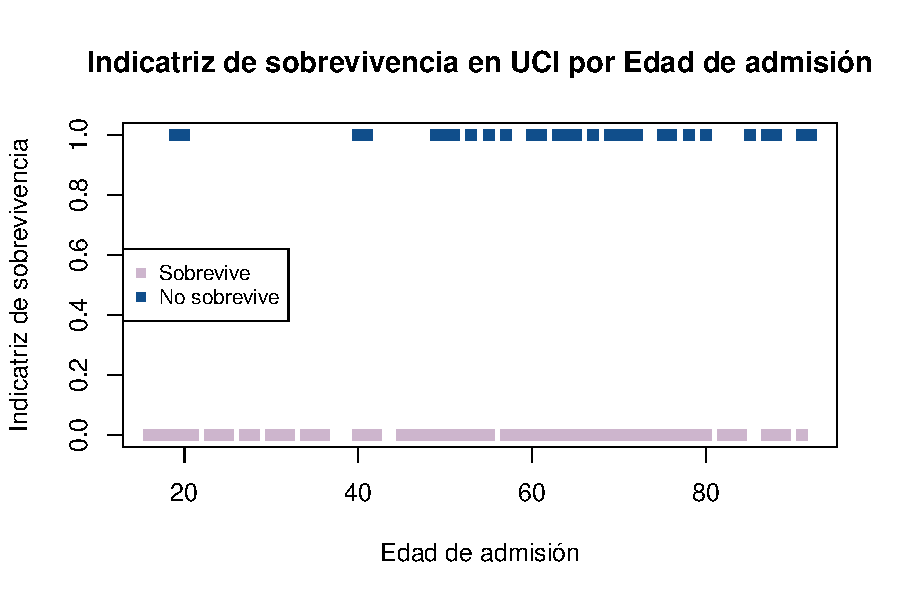
\includegraphics[width=\maxwidth]{figure/unnamed-chunk-2-1} 
\begin{kframe}\begin{alltt}
\hlkwd{print}\hlstd{(}\hlkwd{survfit}\hlstd{(my.surv.object} \hlopt{~} \hlnum{1}\hlstd{),} \hlkwc{print.rmean}\hlstd{=}\hlnum{TRUE}\hlstd{)}
\end{alltt}
\begin{verbatim}
## Call: survfit(formula = my.surv.object ~ 1)
## 
##          n     events     *rmean *se(rmean)     median    0.95LCL 
##   1.00e+03   9.16e+02   3.35e+00   9.67e-02   2.21e+00   2.05e+00 
##    0.95UCL 
##   2.49e+00 
##     * restricted mean with upper limit =  10
\end{verbatim}
\end{kframe}
\end{knitrout}


\end{itemize}

\subsection*{Pregunta 2} 
\begin{itemize}
\item[a)] \textbf{Solución}\\
$$ F(y) = 1-\frac{1}{(1+y)^{\alpha}}$$
\item[b)] \textbf{Solución}\\
$$S(y)=\frac{1}{(1+y)^{\alpha}}$$
\item[c)] \textbf{Solución}\\
$$ h(y)=\frac{\alpha}{1+y}$$
\item[d)] \textbf{Solución}\\
$$\hat{\alpha}_{EMV}=\frac{\sum_{i=1}^{n}{\nu_{i}}}{\sum_{i=1}^{n}{ln(1+y_{i})}}$$
\end{itemize}

\subsection*{Pregunta 3} 
\begin{itemize} 
\item[a)] \textbf{Solución}\\
$$H(t)=ln(1+(t/\alpha)^{\beta})$$
\item[b)] \textbf{Solución}\\ 
$$S(t)=[1+(t/\alpha)^{\beta}]^{-1}$$
\item[c)] \textbf{Solución}\\ 
$$f(t)=\frac{(\beta/\alpha)(t/\alpha)^{\beta-1}}{[1+(t/\alpha)^{\beta}]^{2}}$$
\item[d)] \textbf{Solución}\\
$$F(t)=1-[1+(t/\alpha)^{\beta}]^{-1}$$
\end{itemize}

\subsection*{Pregunta 4} 

\begin{itemize} 

\item[a)] \textbf{Solución}\\


\begin{knitrout}
\definecolor{shadecolor}{rgb}{0.969, 0.969, 0.969}\color{fgcolor}\begin{kframe}
\begin{alltt}
\hlstd{GRUPO1}\hlkwb{<-}\hlkwd{rbind}\hlstd{(}\hlkwd{c}\hlstd{(}\hlnum{12.3}\hlstd{,}\hlnum{0}\hlstd{),}\hlkwd{c}\hlstd{(}\hlnum{5.4}\hlstd{,}\hlnum{1}\hlstd{),}\hlkwd{c}\hlstd{(}\hlnum{8.2}\hlstd{,}\hlnum{1}\hlstd{),}\hlkwd{c}\hlstd{(}\hlnum{12.2}\hlstd{,}\hlnum{0}\hlstd{),}\hlkwd{c}\hlstd{(}\hlnum{11.8}\hlstd{,}\hlnum{1}\hlstd{),}\hlkwd{c}\hlstd{(}\hlnum{10}\hlstd{,}\hlnum{1}\hlstd{),}\hlkwd{c}\hlstd{(}\hlnum{5.7}\hlstd{,}\hlnum{1}\hlstd{),}\hlkwd{c}\hlstd{(}\hlnum{9.8}\hlstd{,}\hlnum{1}\hlstd{),}
              \hlkwd{c}\hlstd{(}\hlnum{2.6}\hlstd{,}\hlnum{1}\hlstd{),}\hlkwd{c}\hlstd{(}\hlnum{11}\hlstd{,}\hlnum{1}\hlstd{),}\hlkwd{c}\hlstd{(}\hlnum{9.2}\hlstd{,}\hlnum{1}\hlstd{),}\hlkwd{c}\hlstd{(}\hlnum{12.1}\hlstd{,}\hlnum{0}\hlstd{),}\hlkwd{c}\hlstd{(}\hlnum{6.6}\hlstd{,}\hlnum{1}\hlstd{),}\hlkwd{c}\hlstd{(}\hlnum{2.2}\hlstd{,}\hlnum{1}\hlstd{),}\hlkwd{c}\hlstd{(}\hlnum{1.8}\hlstd{,}\hlnum{1}\hlstd{),}\hlkwd{c}\hlstd{(}\hlnum{10.2}\hlstd{,}\hlnum{1}\hlstd{),}
              \hlkwd{c}\hlstd{(}\hlnum{10.7}\hlstd{,}\hlnum{1}\hlstd{),}\hlkwd{c}\hlstd{(}\hlnum{11.1}\hlstd{,}\hlnum{1}\hlstd{),}\hlkwd{c}\hlstd{(}\hlnum{5.3}\hlstd{,}\hlnum{1}\hlstd{),}\hlkwd{c}\hlstd{(}\hlnum{3.5}\hlstd{,}\hlnum{1}\hlstd{),}\hlkwd{c}\hlstd{(}\hlnum{9.2}\hlstd{,}\hlnum{1}\hlstd{),}\hlkwd{c}\hlstd{(}\hlnum{2.5}\hlstd{,}\hlnum{1}\hlstd{),}\hlkwd{c}\hlstd{(}\hlnum{8.7}\hlstd{,}\hlnum{1}\hlstd{),}\hlkwd{c}\hlstd{(}\hlnum{3.8}\hlstd{,}\hlnum{1}\hlstd{),}\hlkwd{c}\hlstd{(}\hlnum{3}\hlstd{,}\hlnum{1}\hlstd{))}

\hlstd{GRUPO2}\hlkwb{<-}\hlkwd{cbind}\hlstd{(}\hlkwd{c}\hlstd{(}\hlnum{5.8}\hlstd{,}\hlnum{2.9}\hlstd{,}\hlnum{8.4}\hlstd{,}\hlnum{8.3}\hlstd{,}\hlnum{9.1}\hlstd{,}\hlnum{4.2}\hlstd{,}\hlnum{4.1}\hlstd{,}\hlnum{1.8}\hlstd{,}\hlnum{3.1}\hlstd{,}\hlnum{11.4}\hlstd{,}\hlnum{2.4}\hlstd{,}\hlnum{1.4}\hlstd{,}\hlnum{5.9}\hlstd{,}\hlnum{1.6}\hlstd{,}\hlnum{2.8}\hlstd{,}\hlnum{4.9}\hlstd{,}\hlnum{3.5}\hlstd{,}\hlnum{6.5}\hlstd{,}
                \hlnum{9.9}\hlstd{,}\hlnum{3.6}\hlstd{,}\hlnum{5.2}\hlstd{,}\hlnum{8.8}\hlstd{,}\hlnum{7.8}\hlstd{,}\hlnum{4.7}\hlstd{,}\hlnum{3.9}\hlstd{),}\hlkwd{rep}\hlstd{(}\hlnum{1}\hlstd{,}\hlnum{25}\hlstd{))}

\hlcom{#GRUPO 1}

\hlstd{my.surv.object}\hlkwb{<-}\hlkwd{Surv}\hlstd{(}\hlkwc{time}\hlstd{=GRUPO1[,}\hlnum{1}\hlstd{],}\hlkwc{event} \hlstd{= GRUPO1[,}\hlnum{2}\hlstd{],} \hlkwc{type} \hlstd{=} \hlstr{"right"}\hlstd{)}

\hlkwd{survfit}\hlstd{(my.surv.object} \hlopt{~} \hlnum{1}\hlstd{,}\hlkwc{conf.type}\hlstd{=}\hlstr{"plain"}\hlstd{,} \hlkwc{conf.int}\hlstd{=}\hlnum{0.90}\hlstd{)}
\end{alltt}
\begin{verbatim}
## Call: survfit(formula = my.surv.object ~ 1, conf.type = "plain", conf.int = 0.9)
## 
##      n events median 0.9LCL 0.9UCL 
##   25.0   22.0    8.7    5.4   10.0
\end{verbatim}
\begin{alltt}
\hlstd{my.fit1}\hlkwb{<-}\hlkwd{survfit}\hlstd{(my.surv.object} \hlopt{~} \hlnum{1}\hlstd{)}
\hlkwd{str}\hlstd{(my.fit1)}
\end{alltt}
\begin{verbatim}
## List of 17
##  $ n         : int 25
##  $ time      : num [1:24] 1.8 2.2 2.5 2.6 3 3.5 3.8 5.3 5.4 5.7 ...
##  $ n.risk    : num [1:24] 25 24 23 22 21 20 19 18 17 16 ...
##  $ n.event   : num [1:24] 1 1 1 1 1 1 1 1 1 1 ...
##  $ n.censor  : num [1:24] 0 0 0 0 0 0 0 0 0 0 ...
##  $ surv      : num [1:24] 0.96 0.92 0.88 0.84 0.8 0.76 0.72 0.68 0.64 0.6 ...
##  $ std.err   : num [1:24] 0.0408 0.059 0.0739 0.0873 0.1 ...
##  $ cumhaz    : num [1:24] 0.04 0.0817 0.1251 0.1706 0.2182 ...
##  $ std.chaz  : num [1:24] 0.04 0.0578 0.0723 0.0854 0.0978 ...
##  $ start.time: num 0
##  $ type      : chr "right"
##  $ logse     : logi TRUE
##  $ conf.int  : num 0.95
##  $ conf.type : chr "log"
##  $ lower     : num [1:24] 0.886 0.82 0.761 0.708 0.658 ...
##  $ upper     : num [1:24] 1 1 1 0.997 0.973 ...
##  $ call      : language survfit(formula = my.surv.object ~ 1)
##  - attr(*, "class")= chr "survfit"
\end{verbatim}
\begin{alltt}
\hlcom{#summary(my.fit1)}

\hlkwd{plot}\hlstd{(my.fit1,} \hlkwc{main}\hlstd{=}\hlstr{"Kaplan-Meier estimate Group 1"}\hlstd{,}
     \hlkwc{xlab}\hlstd{=}\hlstr{"time"}\hlstd{,} \hlkwc{ylab}\hlstd{=}\hlstr{"survival function"}\hlstd{,}\hlkwc{mark.time}\hlstd{=T)}
\end{alltt}
\end{kframe}
\includegraphics[width=\maxwidth]{figure/unnamed-chunk-3-1} 
\begin{kframe}\begin{alltt}
\hlkwd{print}\hlstd{(}\hlkwd{survfit}\hlstd{(my.surv.object} \hlopt{~} \hlnum{1}\hlstd{),} \hlkwc{print.rmean}\hlstd{=}\hlnum{TRUE}\hlstd{)}
\end{alltt}
\begin{verbatim}
## Call: survfit(formula = my.surv.object ~ 1)
## 
##          n     events     *rmean *se(rmean)     median    0.95LCL 
##     25.000     22.000      7.568      0.718      8.700      5.400 
##    0.95UCL 
##     10.700 
##     * restricted mean with upper limit =  12.3
\end{verbatim}
\begin{alltt}
\hlcom{#GRUPO 2}
\hlstd{my.surv.object}\hlkwb{<-}\hlkwd{Surv}\hlstd{(}\hlkwc{time}\hlstd{=GRUPO2[,}\hlnum{1}\hlstd{],}\hlkwc{event} \hlstd{= GRUPO2[,}\hlnum{2}\hlstd{],} \hlkwc{type} \hlstd{=} \hlstr{"right"}\hlstd{)}

\hlkwd{survfit}\hlstd{(my.surv.object} \hlopt{~} \hlnum{1}\hlstd{,}\hlkwc{conf.type}\hlstd{=}\hlstr{"plain"}\hlstd{,} \hlkwc{conf.int}\hlstd{=}\hlnum{0.90}\hlstd{)}
\end{alltt}
\begin{verbatim}
## Call: survfit(formula = my.surv.object ~ 1, conf.type = "plain", conf.int = 0.9)
## 
##      n events median 0.9LCL 0.9UCL 
##   25.0   25.0    4.7    3.6    5.9
\end{verbatim}
\begin{alltt}
\hlstd{my.fit2}\hlkwb{<-}\hlkwd{survfit}\hlstd{(my.surv.object} \hlopt{~} \hlnum{1}\hlstd{)}
\hlkwd{str}\hlstd{(my.fit2)}
\end{alltt}
\begin{verbatim}
## List of 17
##  $ n         : int 25
##  $ time      : num [1:25] 1.4 1.6 1.8 2.4 2.8 2.9 3.1 3.5 3.6 3.9 ...
##  $ n.risk    : num [1:25] 25 24 23 22 21 20 19 18 17 16 ...
##  $ n.event   : num [1:25] 1 1 1 1 1 1 1 1 1 1 ...
##  $ n.censor  : num [1:25] 0 0 0 0 0 0 0 0 0 0 ...
##  $ surv      : num [1:25] 0.96 0.92 0.88 0.84 0.8 0.76 0.72 0.68 0.64 0.6 ...
##  $ std.err   : num [1:25] 0.0408 0.059 0.0739 0.0873 0.1 ...
##  $ cumhaz    : num [1:25] 0.04 0.0817 0.1251 0.1706 0.2182 ...
##  $ std.chaz  : num [1:25] 0.04 0.0578 0.0723 0.0854 0.0978 ...
##  $ start.time: num 0
##  $ type      : chr "right"
##  $ logse     : logi TRUE
##  $ conf.int  : num 0.95
##  $ conf.type : chr "log"
##  $ lower     : num [1:25] 0.886 0.82 0.761 0.708 0.658 ...
##  $ upper     : num [1:25] 1 1 1 0.997 0.973 ...
##  $ call      : language survfit(formula = my.surv.object ~ 1)
##  - attr(*, "class")= chr "survfit"
\end{verbatim}
\begin{alltt}
\hlcom{#summary(my.fit2)}

\hlkwd{plot}\hlstd{(my.fit2,} \hlkwc{main}\hlstd{=}\hlstr{"Kaplan-Meier estimate  Group 2"}\hlstd{,}
     \hlkwc{xlab}\hlstd{=}\hlstr{"time"}\hlstd{,} \hlkwc{ylab}\hlstd{=}\hlstr{"survival function"}\hlstd{,}\hlkwc{mark.time}\hlstd{=T)}
\end{alltt}
\end{kframe}
\includegraphics[width=\maxwidth]{figure/unnamed-chunk-3-2} 
\begin{kframe}\begin{alltt}
\hlkwd{print}\hlstd{(}\hlkwd{survfit}\hlstd{(my.surv.object} \hlopt{~} \hlnum{1}\hlstd{),} \hlkwc{print.rmean}\hlstd{=}\hlnum{TRUE}\hlstd{)}
\end{alltt}
\begin{verbatim}
## Call: survfit(formula = my.surv.object ~ 1)
## 
##          n     events     *rmean *se(rmean)     median    0.95LCL 
##     25.000     25.000      5.280      0.551      4.700      3.600 
##    0.95UCL 
##      7.800 
##     * restricted mean with upper limit =  11.4
\end{verbatim}
\end{kframe}
\end{knitrout}

\item[b)] \textbf{Solución}\\ 
\end{itemize}

\begin{knitrout}
\definecolor{shadecolor}{rgb}{0.969, 0.969, 0.969}\color{fgcolor}\begin{kframe}
\begin{alltt}
\hlkwd{par}\hlstd{(}\hlkwc{mfrow}\hlstd{=}\hlkwd{c}\hlstd{(}\hlnum{1}\hlstd{,}\hlnum{2}\hlstd{))}

\hlkwd{plot}\hlstd{(my.fit1,} \hlkwc{main}\hlstd{=}\hlstr{"Kaplan-Meier estimate Group 1"}\hlstd{,}
     \hlkwc{xlab}\hlstd{=}\hlstr{"time"}\hlstd{,} \hlkwc{ylab}\hlstd{=}\hlstr{"survival function"}\hlstd{,}\hlkwc{mark.time}\hlstd{=T)}

\hlkwd{plot}\hlstd{(my.fit2,} \hlkwc{main}\hlstd{=}\hlstr{"Kaplan-Meier estimate Group 2"}\hlstd{,}
     \hlkwc{xlab}\hlstd{=}\hlstr{"time"}\hlstd{,} \hlkwc{ylab}\hlstd{=}\hlstr{"survival function"}\hlstd{,}\hlkwc{mark.time}\hlstd{=T)}
\end{alltt}
\end{kframe}
\includegraphics[width=\maxwidth]{figure/unnamed-chunk-4-1} 
\begin{kframe}\begin{alltt}
\hlstd{DATA}\hlkwb{<-}\hlkwd{rbind}\hlstd{(}\hlkwd{cbind}\hlstd{(GRUPO1,}\hlkwd{rep}\hlstd{(}\hlnum{3}\hlstd{,}\hlnum{25}\hlstd{)),}\hlkwd{cbind}\hlstd{(GRUPO2,}\hlkwd{rep}\hlstd{(}\hlnum{2}\hlstd{,}\hlnum{25}\hlstd{)))}
\hlkwd{colnames}\hlstd{(DATA)}\hlkwb{<-}\hlkwd{c}\hlstd{(}\hlstr{"tiempos"}\hlstd{,}\hlstr{"censura"}\hlstd{,}\hlstr{"trat"}\hlstd{)}
\hlstd{DATA}\hlkwb{<-}\hlkwd{data.frame}\hlstd{(DATA)}
\hlkwd{survdiff}\hlstd{(}\hlkwd{Surv}\hlstd{(tiempos, censura)}\hlopt{~}\hlstd{trat,} \hlkwc{data}\hlstd{=DATA)}
\end{alltt}
\begin{verbatim}
## Call:
## survdiff(formula = Surv(tiempos, censura) ~ trat, data = DATA)
## 
##         N Observed Expected (O-E)^2/E (O-E)^2/V
## trat=2 25       25     16.2      4.76      7.99
## trat=3 25       22     30.8      2.51      7.99
## 
##  Chisq= 8  on 1 degrees of freedom, p= 0.005
\end{verbatim}
\begin{alltt}
\hlcom{#Las curvas difieren. (investigar test)}
\end{alltt}
\end{kframe}
\end{knitrout}

\subsection*{Pregunta 5}
\textbf{Solución}\\ 

\begin{itemize}
\item[a)] Verdadero.
\item[b)] Verdadero.
\item[c)] Falso. El Kaplan-Meier posee una gráfica escalonada usualmente.
\item[d)] Falso. Está entre 0 y 1.
\item[e)] Verdadero.
\item[f)] Falso. La media del tiempo de sobrevivencia para el grupo 1 es mayor que para el grupo 2. 
\item[g)] Falso. Cuyos tiempos de sobrevivencia son mayores a seis semanas.
\item[h)] Falso. Serían 13 personas.
\item[i)] Verdadero.
\end{itemize}

\subsection*{Pregunta 7} \textbf{Solución}\\ 
\begin{itemize}
\item[a)] \textbf{Solución}\\ 

Para placebo:

\begin{center}
\begin{tabular}{|l|l|l|l|l|}
\hline
$t_{k}$ & $d_{k}$& $q_{k}$ & $n_{k}$ & $\hat{S}(t)$\\
\hline
0 & 0 & 0& 8 & 1\\
\hline
1 & 2 & 1 & 8 & $(1-\frac{2}{8})$\\
\hline
2&2&0&5&$(1-\frac{2}{8})(1-\frac{2}{5})$\\
\hline 
3&2&1&5&$(1-\frac{2}{8})(1-\frac{2}{5}(1-\frac{2}{5})$\\
\hline
\end{tabular}
\end{center}

Para tratamiento:

\begin{center}
\begin{tabular}{|l|l|l|l|l|}
\hline
$t_{k}$ & $d_{k}$& $q_{k}$ & $n_{k}$ & $\hat{S}(t)$\\
\hline
0 & 0 & 0& 9 & 1\\
\hline
1&1&0&9&$(1-\frac{1}{9})$\\
\hline
2&2&1&8&$(1-\frac{1}{9})(1-\frac{2}{8})$\\
\hline
3&2&0&5&$(1-\frac{1}{9})(1-\frac{2}{8})(1-\frac{2}{5})$\\
\hline
4&1&0&3&$(1-\frac{1}{9})(1-\frac{2}{8})(1-\frac{2}{5})(1-\frac{1}{3}$\\
\hline
5&1&1&2& $(1-\frac{1}{9})(1-\frac{2}{8})(1-\frac{2}{5})(1-\frac{1}{3}(1-\frac{1}{2}$\\
\hline
\end{tabular}
\end{center}

O también: 
\begin{knitrout}
\definecolor{shadecolor}{rgb}{0.969, 0.969, 0.969}\color{fgcolor}\begin{kframe}
\begin{alltt}
\hlstd{datos}\hlkwb{<-}\hlkwd{cbind}\hlstd{(}\hlkwd{c}\hlstd{(}\hlnum{1}\hlstd{,}\hlnum{1}\hlstd{,}\hlnum{1}\hlstd{,}\hlnum{2}\hlstd{,}\hlnum{2}\hlstd{,}\hlnum{3}\hlstd{,}\hlnum{3}\hlstd{,}\hlnum{3}\hlstd{,}\hlnum{1}\hlstd{,}\hlnum{2}\hlstd{,}\hlnum{2}\hlstd{,}\hlnum{2}\hlstd{,}\hlnum{3}\hlstd{,}\hlnum{3}\hlstd{,}\hlnum{4}\hlstd{,}\hlnum{5}\hlstd{,}\hlnum{5}\hlstd{),}
             \hlkwd{c}\hlstd{(}\hlnum{1}\hlstd{,}\hlnum{1}\hlstd{,}\hlnum{0}\hlstd{,}\hlnum{1}\hlstd{,}\hlnum{1}\hlstd{,}\hlnum{1}\hlstd{,}\hlnum{1}\hlstd{,}\hlnum{0}\hlstd{,}\hlnum{1}\hlstd{,}\hlnum{1}\hlstd{,}\hlnum{0}\hlstd{,}\hlnum{1}\hlstd{,}\hlnum{1}\hlstd{,}\hlnum{1}\hlstd{,}\hlnum{1}\hlstd{,}\hlnum{1}\hlstd{,}\hlnum{0}\hlstd{),}\hlkwd{c}\hlstd{(}\hlkwd{rep}\hlstd{(}\hlnum{0}\hlstd{,}\hlnum{8}\hlstd{),}\hlkwd{rep}\hlstd{(}\hlnum{1}\hlstd{,}\hlnum{9}\hlstd{)))}

\hlkwd{head}\hlstd{(datos)}
\end{alltt}
\begin{verbatim}
##      [,1] [,2] [,3]
## [1,]    1    1    0
## [2,]    1    1    0
## [3,]    1    0    0
## [4,]    2    1    0
## [5,]    2    1    0
## [6,]    3    1    0
\end{verbatim}
\begin{alltt}
\hlkwd{library}\hlstd{(survival)}
\hlstd{Sp}\hlkwb{<-}\hlkwd{Surv}\hlstd{(datos[}\hlnum{1}\hlopt{:}\hlnum{8}\hlstd{,}\hlnum{1}\hlstd{],datos[}\hlnum{1}\hlopt{:}\hlnum{8}\hlstd{,}\hlnum{2}\hlstd{])}
\hlstd{Sp}
\end{alltt}
\begin{verbatim}
## [1] 1  1  1+ 2  2  3  3  3+
\end{verbatim}
\begin{alltt}
\hlstd{St}\hlkwb{<-}\hlkwd{Surv}\hlstd{(datos[}\hlnum{9}\hlopt{:}\hlnum{17}\hlstd{,}\hlnum{1}\hlstd{],datos[}\hlnum{9}\hlopt{:}\hlnum{17}\hlstd{,}\hlnum{2}\hlstd{])}
\hlstd{St}
\end{alltt}
\begin{verbatim}
## [1] 1  2  2+ 2  3  3  4  5  5+
\end{verbatim}
\begin{alltt}
\hlstd{spfit}\hlkwb{<-}\hlkwd{survfit}\hlstd{(Sp}\hlopt{~}\hlnum{1}\hlstd{,)}
\hlstd{stfit}\hlkwb{<-}\hlkwd{survfit}\hlstd{(St}\hlopt{~}\hlnum{1}\hlstd{,)}


\hlkwd{summary}\hlstd{(spfit)}
\end{alltt}
\begin{verbatim}
## Call: survfit(formula = Sp ~ 1)
## 
##  time n.risk n.event survival std.err lower 95% CI upper 95% CI
##     1      8       2     0.75   0.153       0.5027        1.000
##     2      5       2     0.45   0.188       0.1982        1.000
##     3      3       2     0.15   0.138       0.0248        0.906
\end{verbatim}
\begin{alltt}
\hlkwd{summary}\hlstd{(stfit)}
\end{alltt}
\begin{verbatim}
## Call: survfit(formula = St ~ 1)
## 
##  time n.risk n.event survival std.err lower 95% CI upper 95% CI
##     1      9       1    0.889   0.105       0.7056        1.000
##     2      8       2    0.667   0.157       0.4200        1.000
##     3      5       2    0.400   0.174       0.1707        0.938
##     4      3       1    0.267   0.159       0.0829        0.858
##     5      2       1    0.133   0.123       0.0218        0.817
\end{verbatim}
\begin{alltt}
\hlkwd{summary}\hlstd{(spfit,}\hlkwc{time}\hlstd{=}\hlnum{2}\hlstd{)}
\end{alltt}
\begin{verbatim}
## Call: survfit(formula = Sp ~ 1)
## 
##  time n.risk n.event survival std.err lower 95% CI upper 95% CI
##     2      5       4     0.45   0.188        0.198            1
\end{verbatim}
\begin{alltt}
\hlkwd{summary}\hlstd{(stfit,}\hlkwc{time}\hlstd{=}\hlnum{2}\hlstd{)}
\end{alltt}
\begin{verbatim}
## Call: survfit(formula = St ~ 1)
## 
##  time n.risk n.event survival std.err lower 95% CI upper 95% CI
##     2      8       3    0.667   0.157         0.42            1
\end{verbatim}
\end{kframe}
\end{knitrout}


\item[b)] \textbf{Solución}\\ 

\begin{knitrout}
\definecolor{shadecolor}{rgb}{0.969, 0.969, 0.969}\color{fgcolor}\begin{kframe}
\begin{alltt}
\hlstd{sexp}\hlkwb{<-}\hlkwd{survreg}\hlstd{(}\hlkwd{Surv}\hlstd{(datos[,}\hlnum{1}\hlstd{],datos[,}\hlnum{2}\hlstd{])}\hlopt{~}\hlstd{datos[,}\hlnum{3}\hlstd{],}\hlkwc{dist}\hlstd{=}\hlstr{"exponential"}\hlstd{)}
\hlstd{sexp}
\end{alltt}
\begin{verbatim}
## Call:
## survreg(formula = Surv(datos[, 1], datos[, 2]) ~ datos[, 3], 
##     dist = "exponential")
## 
## Coefficients:
## (Intercept)  datos[, 3] 
##   0.9808293   0.3690975 
## 
## Scale fixed at 1 
## 
## Loglik(model)= -28.3   Loglik(intercept only)= -28.6
## 	Chisq= 0.43 on 1 degrees of freedom, p= 0.51 
## n= 17
\end{verbatim}
\begin{alltt}
\hlkwd{summary}\hlstd{(sexp)}
\end{alltt}
\begin{verbatim}
## 
## Call:
## survreg(formula = Surv(datos[, 1], datos[, 2]) ~ datos[, 3], 
##     dist = "exponential")
##             Value Std. Error    z     p
## (Intercept) 0.981      0.408 2.40 0.016
## datos[, 3]  0.369      0.556 0.66 0.507
## 
## Scale fixed at 1 
## 
## Exponential distribution
## Loglik(model)= -28.3   Loglik(intercept only)= -28.6
## 	Chisq= 0.43 on 1 degrees of freedom, p= 0.51 
## Number of Newton-Raphson Iterations: 3 
## n= 17
\end{verbatim}
\begin{alltt}
\hlcom{#El valor p es igual a 0.5, utilizando un 5%, no sería significativo el tratamiento}
\hlcom{#para explicar los tiempos de sobrevivencia}
\hlkwd{AIC}\hlstd{(sexp)}
\end{alltt}
\begin{verbatim}
## [1] 60.66893
\end{verbatim}
\end{kframe}
\end{knitrout}

\item[c)] \textbf{Solución}\\ 


\begin{knitrout}
\definecolor{shadecolor}{rgb}{0.969, 0.969, 0.969}\color{fgcolor}\begin{kframe}
\begin{alltt}
\hlstd{fit_0}\hlkwb{<-}\hlkwd{coxph}\hlstd{(}\hlkwd{Surv}\hlstd{(datos[,}\hlnum{1}\hlstd{],datos[,}\hlnum{2}\hlstd{])}\hlopt{~}\hlstd{datos[,}\hlnum{3}\hlstd{])}
\hlkwd{summary}\hlstd{(fit_0)}
\end{alltt}
\begin{verbatim}
## Call:
## coxph(formula = Surv(datos[, 1], datos[, 2]) ~ datos[, 3])
## 
##   n= 17, number of events= 13 
## 
##               coef exp(coef) se(coef)      z Pr(>|z|)
## datos[, 3] -0.6671    0.5132   0.6090 -1.095    0.273
## 
##            exp(coef) exp(-coef) lower .95 upper .95
## datos[, 3]    0.5132      1.949    0.1556     1.693
## 
## Concordance= 0.603  (se = 0.085 )
## Likelihood ratio test= 1.2  on 1 df,   p=0.3
## Wald test            = 1.2  on 1 df,   p=0.3
## Score (logrank) test = 1.24  on 1 df,   p=0.3
\end{verbatim}
\begin{alltt}
\hlcom{#Al ajustar el modelo de riesgos proporcionales, se obtiene un valor-p para el }
\hlcom{#tratamiento de 0.27, es decir, aún no es significativo.}
\hlcom{#la exp(coeftrat)=0.5132, es decir, cuando paso del placebo al tratamiento, los }
\hlcom{#riesgos disminuyen un 48% aproximadamente. }
\hlcom{#El intervalo de confianza al 95% es (0.1556,1.693), el cual contiene al 1, }
\hlcom{#por lo tanto, no se puede rechazar que el efecto del tratamiento sea nulo.}

\hlkwd{cox.zph}\hlstd{(fit_0,} \hlkwc{transform}\hlstd{=}\hlstr{"km"}\hlstd{,} \hlkwc{global}\hlstd{=}\hlnum{TRUE}\hlstd{)}
\end{alltt}
\begin{verbatim}
##               rho  chisq     p
## datos[, 3] 0.0172 0.0038 0.951
\end{verbatim}
\begin{alltt}
\hlcom{#Obtenemos un valor-p de 0.951, es decir, no rechazamos H0 (que los riesgos son proporcionales)}
\end{alltt}
\end{kframe}
\end{knitrout}

\end{itemize}
\subsection*{Pregunta 8}

\begin{itemize}

\item[a)]  \textbf{Solución}\\ 
Trabajar la expresión $HR(t,x_{1},x_{2}))$ y llegar a que no depende del tiempo (se cancelan las funciones que dependen  de $t$).
\item[b)]  \textbf{Solución}\\ 
$$HR_{sexo}(t,x_{1}=1,x_{2}=0)=e^{\hat{\beta}_{1}}=e^{-0.3}=1.35$$
Los hombres tienen un $35$ por ciento más de riesgo en comparación a las mujeres.\\
$$HR_{peso}(t,x_{1}=70,x_{2}=69)=e^{\hat{\beta}_{2}}=e^{0.77}=2.16$$
Por cada kilo de aumento en el peso, el riesgo aumenta un 116 por ciento.\\
$$HR_{tratamiento}(t,x_{1}=1,x_{2}=0)=e^{\hat{\beta}_{3}}=e^{-0.18}=0.83$$
El tratamiento baja el riesgo en un $17$ por ciento.

\item[c)] \textbf{Solución}\\ 
Falso. Las funciones de riesgo están relacionadas de manera multiplicativa.
\item[d)] \textbf{Solución}\\ 
Verdadero. La razón de riesgo es constante sobre el tiempo de sobrevida.  

\end{itemize}

\subsection*{Pregunta 9}
\begin{itemize}
\item[a)] \textbf{Solución}\\ 
Los predictores con un efecto significativo sobre la sobrevivencia de los pacientes son: Karnofsky performance scale, cell type, therapy y la interración de Prio therapy con la therapy actual. Esto se deduce de los resultados del test de Wald.
\item[b)] \textbf{Solución}\\ 
$e^{0.56662}=1.7623$. Los pacientes en el grupo de terapia test un $76$ por ciento más de riesgo de morir en relación a los que reciben la terapia estándar.
\item[c)] \textbf{Solución}\\ 
$e^{-0.033}=0.9675$ es un factor protector, de hecho el riesgo de morir disminuye en un $3.2$ por ciento por cada unidad de aumento en el kps.
\item[d)] \textbf{Solución}\\ 
$e^{-0.87579}=0.4165$. Los pacientes que recibieron terapia previa y ahora están recibiendo la quimioterapia de prueba, tienen un $58.35$ por ciento menos de riesgos de morir.
\item[e)] \textbf{Solución}\\ 
$e^{0.78356}=2.189252$. Los pacientes con celulas tipo adeno tienen un $118$ por ciento más de riesgo de morir en relación a los que tienen células large. (Factor de riesgo) \\
Los pacientes con células small tienen un $61.98$ por ciento más de riesgo de morir en relación a los que tienen células large. (Factor de riesgo)\\
$e^{-0.4077}=0.6652$. Los pacientes con células tipo suqmous tienen un $33.48$ por ciento menos de riesgo de morir en relación a los que tienen células large. (Factor protector)
\item[f)] \textbf{Solución}\\ 
Se recomienda aplicar la quimioterapia test sólo a los pacientes que recibieron una terapia previa.

\end{itemize}


\subsection*{Pregunta 10}
\textbf{Solución}\\

\begin{knitrout}
\definecolor{shadecolor}{rgb}{0.969, 0.969, 0.969}\color{fgcolor}\begin{kframe}
\begin{alltt}
\hlstd{Fan}\hlkwb{<-}\hlkwd{read.table}\hlstd{(}\hlstr{'Fan.txt'}\hlstd{)}
\hlkwd{colnames}\hlstd{(Fan)}\hlkwb{<-}\hlkwd{c}\hlstd{(}\hlstr{"lifetime"}\hlstd{,}\hlstr{"censor"}\hlstd{)}
\hlstd{Fan[,}\hlnum{1}\hlstd{]}\hlkwb{<-}\hlstd{Fan}\hlopt{$}\hlstd{lifetime}\hlopt{/}\hlnum{1000}

\hlkwd{attach}\hlstd{(Fan)}

\hlkwd{library}\hlstd{(truncnorm)}

\hlcom{# Calcula cantidades fijas}
\hlstd{nu}\hlkwb{=}\hlstd{(censor}\hlopt{==}\hlnum{0}\hlstd{)}\hlopt{*}\hlnum{1}\hlstd{; y}\hlkwb{=}\hlstd{lifetime; n}\hlkwb{=}\hlkwd{length}\hlstd{(nu)}
\hlstd{sum_nu}\hlkwb{=}\hlkwd{sum}\hlstd{(nu)}

\hlcom{# Fija hyper-parámetros}
\hlstd{mu0}\hlkwb{=}\hlnum{0}\hlstd{; sigma02}\hlkwb{=}\hlnum{1000}\hlstd{; alpha0}\hlkwb{=}\hlnum{0.01}\hlstd{; kappa0}\hlkwb{=}\hlnum{0.01}\hlstd{; c}\hlkwb{=}\hlnum{0.1}

\hlcom{# Fija valores iniciales}
\hlstd{alpha}\hlkwb{=}\hlnum{5}\hlstd{; lambda}\hlkwb{=}\hlnum{0.1}
\hlstd{alphaante}\hlkwb{=}\hlstd{alpha; lambdaante}\hlkwb{=}\hlstd{lambda}
\hlstd{nscan}\hlkwb{=}\hlnum{50000}

\hlstd{alphaM}\hlkwb{=}\hlkwd{vector}\hlstd{(}\hlkwc{mode}\hlstd{=}\hlstr{"numeric"}\hlstd{,} \hlkwc{length}\hlstd{=nscan)}
\hlstd{lambdaM}\hlkwb{=}\hlkwd{vector}\hlstd{(}\hlkwc{mode}\hlstd{=}\hlstr{"numeric"}\hlstd{,} \hlkwc{length}\hlstd{=nscan)}
\hlstd{alphaM[}\hlnum{1}\hlstd{]}\hlkwb{=}\hlstd{alpha}
\hlstd{lambdaM[}\hlnum{1}\hlstd{]}\hlkwb{=}\hlstd{lambda}

\hlkwa{for}\hlstd{(i} \hlkwa{in} \hlnum{2}\hlopt{:}\hlstd{nscan)}
\hlstd{\{}

  \hlcom{# Actualización de alpha}
  \hlstd{alphaaste}\hlkwb{=}\hlkwd{rtruncnorm}\hlstd{(}\hlkwc{n}\hlstd{=}\hlnum{1}\hlstd{,} \hlkwc{a}\hlstd{=}\hlnum{0}\hlstd{,} \hlkwc{b}\hlstd{=}\hlnum{Inf}\hlstd{,} \hlkwc{mean}\hlstd{=alphaante,} \hlkwc{sd}\hlstd{=c)}
  \hlstd{logPaste}\hlkwb{=}\hlstd{(alpha0}\hlopt{+}\hlstd{sum_nu}\hlopt{-}\hlnum{1}\hlstd{)}\hlopt{*}\hlkwd{log}\hlstd{(alphaaste)}\hlopt{+} \hlkwd{sum}\hlstd{((alphaaste}\hlopt{-}\hlnum{1}\hlstd{)}\hlopt{*}\hlstd{nu}\hlopt{*}\hlkwd{log}\hlstd{(y)}\hlopt{-}\hlkwd{exp}\hlstd{(lambda)}\hlopt{*}\hlstd{y}\hlopt{^}\hlstd{alphaaste)}\hlopt{-}\hlstd{alphaaste}\hlopt{*}\hlstd{kappa0}
  \hlstd{logPante}\hlkwb{=}\hlstd{(alpha0}\hlopt{+}\hlstd{sum_nu}\hlopt{-}\hlnum{1}\hlstd{)}\hlopt{*}\hlkwd{log}\hlstd{(alphaante)}\hlopt{+} \hlkwd{sum}\hlstd{((alphaante}\hlopt{-}\hlnum{1}\hlstd{)}\hlopt{*}\hlstd{nu}\hlopt{*}\hlkwd{log}\hlstd{(y)}\hlopt{-}\hlkwd{exp}\hlstd{(lambda)}\hlopt{*}\hlstd{y}\hlopt{^}\hlstd{alphaante)}\hlopt{-}\hlstd{alphaante}\hlopt{*}\hlstd{kappa0}
  \hlstd{logJtaste}\hlkwb{=}\hlkwd{log}\hlstd{(}\hlkwd{dtruncnorm}\hlstd{(}\hlkwc{x}\hlstd{=alphaaste,} \hlkwc{a}\hlstd{=}\hlnum{0}\hlstd{,} \hlkwc{b}\hlstd{=}\hlnum{Inf}\hlstd{,} \hlkwc{mean}\hlstd{=alphaante,} \hlkwc{sd}\hlstd{=c))}
  \hlstd{logJtante}\hlkwb{=}\hlkwd{log}\hlstd{(}\hlkwd{dtruncnorm}\hlstd{(}\hlkwc{x}\hlstd{=alphaante,} \hlkwc{a}\hlstd{=}\hlnum{0}\hlstd{,} \hlkwc{b}\hlstd{=}\hlnum{Inf}\hlstd{,} \hlkwc{mean}\hlstd{=alphaaste,} \hlkwc{sd}\hlstd{=c))}
  \hlstd{lnr1}\hlkwb{=}\hlstd{logPaste}\hlopt{-}\hlstd{logJtaste}\hlopt{-}\hlstd{logPante}\hlopt{+}\hlstd{logJtante}
  \hlstd{p1}\hlkwb{=}\hlkwd{exp}\hlstd{(}\hlkwd{min}\hlstd{(lnr1,}\hlnum{0}\hlstd{))}
  \hlstd{u1}\hlkwb{=}\hlkwd{runif}\hlstd{(}\hlnum{1}\hlstd{)}
  \hlkwa{if}\hlstd{(p1}\hlopt{>}\hlstd{u1)\{alpha}\hlkwb{=}\hlstd{alphaaste\}}
  \hlkwa{if}\hlstd{(p1}\hlopt{<=}\hlstd{u1)\{alpha}\hlkwb{=}\hlstd{alphaante\}}
  \hlstd{alphaante}\hlkwb{=}\hlstd{alpha}

  \hlcom{# Actualización de lambda}
  \hlstd{lambdaaste}\hlkwb{=}\hlkwd{rnorm}\hlstd{(}\hlkwc{n}\hlstd{=}\hlnum{1}\hlstd{,} \hlkwc{mean}\hlstd{=lambdaante,} \hlkwc{sd}\hlstd{=c)}
  \hlstd{logPaste}\hlkwb{=}\hlstd{lambdaaste}\hlopt{*}\hlstd{sum_nu}\hlopt{-}\hlkwd{exp}\hlstd{(lambdaaste)}\hlopt{*}\hlkwd{sum}\hlstd{(y}\hlopt{^}\hlstd{alpha)}\hlopt{-}\hlstd{(}\hlnum{0.5}\hlopt{*}\hlstd{(lambdaaste}\hlopt{-}\hlstd{mu0)}\hlopt{^}\hlnum{2}\hlstd{)}\hlopt{/}\hlstd{sigma02}
  \hlstd{logPante}\hlkwb{=}\hlstd{lambdaante}\hlopt{*}\hlstd{sum_nu}\hlopt{-}\hlkwd{exp}\hlstd{(lambdaante)}\hlopt{*}\hlkwd{sum}\hlstd{(y}\hlopt{^}\hlstd{alpha)}\hlopt{-}\hlstd{(}\hlnum{0.5}\hlopt{*}\hlstd{(lambdaante}\hlopt{-}\hlstd{mu0)}\hlopt{^}\hlnum{2}\hlstd{)}\hlopt{/}\hlstd{sigma02}
  \hlstd{lnr2}\hlkwb{=}\hlstd{logPaste}\hlopt{-}\hlstd{logPante}
  \hlstd{p2}\hlkwb{=}\hlkwd{exp}\hlstd{(}\hlkwd{min}\hlstd{(lnr2,}\hlnum{0}\hlstd{))}
  \hlstd{u2}\hlkwb{=}\hlkwd{runif}\hlstd{(}\hlnum{1}\hlstd{)}
  \hlkwa{if}\hlstd{(p2}\hlopt{>}\hlstd{u2)\{lambda}\hlkwb{=}\hlstd{lambdaaste\}}
  \hlkwa{if}\hlstd{(p2}\hlopt{<=}\hlstd{u2)\{lambda}\hlkwb{=}\hlstd{lambdaante\}}
  \hlstd{lambdaante}\hlkwb{=}\hlstd{lambda}

  \hlstd{alphaM[i]}\hlkwb{=}\hlstd{alpha}
  \hlstd{lambdaM[i]}\hlkwb{=}\hlstd{lambda}
\hlstd{\}}

\hlkwd{plot}\hlstd{(alphaM,} \hlkwc{type}\hlstd{=}\hlstr{"l"}\hlstd{)}
\hlkwd{plot}\hlstd{(lambdaM,} \hlkwc{type}\hlstd{=}\hlstr{"l"}\hlstd{)}

\hlkwd{summary}\hlstd{(alphaM)}
\hlkwd{summary}\hlstd{(lambdaM)}

\hlcom{# Muestras desde la posteriori}
\hlstd{indices}\hlkwb{=}\hlkwd{seq}\hlstd{(}\hlnum{2000}\hlstd{,}\hlnum{50000}\hlstd{,}\hlnum{48}\hlstd{)}
\hlstd{alpham}\hlkwb{=}\hlstd{alphaM[indices]}
\hlstd{lambdam}\hlkwb{=}\hlstd{lambdaM[indices]}
\hlkwd{acf}\hlstd{(alpham)}
\hlkwd{acf}\hlstd{(lambdam)}

\hlkwd{hist}\hlstd{(alpham)}
\hlkwd{hist}\hlstd{(lambdam)}
\hlstd{mean.alpha}\hlkwb{=}\hlkwd{mean}\hlstd{(alpham)}
\hlstd{mean.lambda}\hlkwb{=}\hlkwd{mean}\hlstd{(lambdam)}
\hlkwd{exp}\hlstd{(}\hlkwd{mean}\hlstd{(lambdam))}

\hlstd{p025.alpha}\hlkwb{=}\hlkwd{quantile}\hlstd{(alpham,} \hlkwc{probs}\hlstd{=}\hlnum{0.025}\hlstd{)}
\hlstd{p0975.alpha}\hlkwb{=}\hlkwd{quantile}\hlstd{(alpham,} \hlkwc{probs}\hlstd{=}\hlnum{0.975}\hlstd{)}

\hlstd{p025.lambda}\hlkwb{=}\hlkwd{quantile}\hlstd{(lambdam,} \hlkwc{probs}\hlstd{=}\hlnum{0.025}\hlstd{)}
\hlstd{p0975.lambda}\hlkwb{=}\hlkwd{quantile}\hlstd{(lambdam,} \hlkwc{probs}\hlstd{=}\hlnum{0.975}\hlstd{)}

\hlcom{# Función de sobrevivencia}
\hlstd{yy}\hlkwb{=}\hlkwd{seq}\hlstd{(}\hlnum{0}\hlstd{,}\hlnum{2}\hlstd{,}\hlnum{0.01}\hlstd{)}
\hlstd{Sy}\hlkwb{=}\hlkwd{exp}\hlstd{(}\hlopt{-}\hlkwd{exp}\hlstd{(mean.lambda)}\hlopt{*}\hlstd{yy}\hlopt{^}\hlstd{(mean.alpha))}
\hlstd{Sy025}\hlkwb{=}\hlkwd{exp}\hlstd{(}\hlopt{-}\hlkwd{exp}\hlstd{(p025.lambda)}\hlopt{*}\hlstd{yy}\hlopt{^}\hlstd{(p025.alpha))}
\hlstd{Sy0975}\hlkwb{=}\hlkwd{exp}\hlstd{(}\hlopt{-}\hlkwd{exp}\hlstd{(p0975.lambda)}\hlopt{*}\hlstd{yy}\hlopt{^}\hlstd{(p0975.alpha))}
\hlkwd{plot}\hlstd{(yy, Sy,} \hlkwc{type}\hlstd{=}\hlstr{"l"}\hlstd{)}
\hlkwd{lines}\hlstd{(yy, Sy025,} \hlkwc{lty}\hlstd{=}\hlnum{2}\hlstd{,} \hlkwc{col}\hlstd{=}\hlnum{2}\hlstd{)}
\hlkwd{lines}\hlstd{(yy, Sy0975,} \hlkwc{lty}\hlstd{=}\hlnum{2}\hlstd{,} \hlkwc{col}\hlstd{=}\hlnum{2}\hlstd{)}

\hlcom{# Función de riesgo}
\hlstd{hy}\hlkwb{=}\hlstd{mean.alpha}\hlopt{*}\hlstd{yy}\hlopt{^}\hlstd{(mean.alpha}\hlopt{-}\hlnum{1}\hlstd{)}\hlopt{*}\hlkwd{exp}\hlstd{(mean.lambda)}
\hlstd{hy025}\hlkwb{=}\hlstd{p025.alpha}\hlopt{*}\hlstd{yy}\hlopt{^}\hlstd{(p025.alpha}\hlopt{-}\hlnum{1}\hlstd{)}\hlopt{*}\hlkwd{exp}\hlstd{(p025.lambda)}
\hlstd{hy0975}\hlkwb{=}\hlstd{p0975.alpha}\hlopt{*}\hlstd{yy}\hlopt{^}\hlstd{(p0975.alpha}\hlopt{-}\hlnum{1}\hlstd{)}\hlopt{*}\hlkwd{exp}\hlstd{(p0975.lambda)}
\hlkwd{plot}\hlstd{(yy, hy,} \hlkwc{type}\hlstd{=}\hlstr{"l"}\hlstd{)}
\hlkwd{lines}\hlstd{(yy, hy025,} \hlkwc{lty}\hlstd{=}\hlnum{2}\hlstd{,} \hlkwc{col}\hlstd{=}\hlnum{2}\hlstd{)}
\hlkwd{lines}\hlstd{(yy, hy0975,} \hlkwc{lty}\hlstd{=}\hlnum{2}\hlstd{,} \hlkwc{col}\hlstd{=}\hlnum{2}\hlstd{)}
\end{alltt}
\end{kframe}
\end{knitrout}
\subsection*{Pregunta 11}
Se puede definir de manera general:
$$W(\omega_{0})=W=2[l(\hat{w},\hat{\lambda})-l(\omega_{0},\hat{\lambda}_{\omega_{0}})]$$ 
Donde $l(\hat{w},\hat{\lambda})$ corresponde a la estimación de máxima verosimilitud usual y $l(\omega_{0},\hat{\lambda}_{\omega_{0}})$ corresponde a la estimación de máxima verosimilitud restringida a la hipótesis nula ($\omega=\omega_{0}$). Bajo la hipótesis nula, el estadístico $W(\omega_{0})=W$ tiene aproximadamente una distribución chi-cuadrado, con $p_{\omega}=dim(\omega)$ grados de libertad. Si la distribución asintótica fuera exacta, se tendría que $E(W)=p_{\omega}$, sin embargo, se tiene por el \textit{Factor de corrección de Barlett} que:
$$E(W)=p_{\omega}[1+\frac{c}{n}+o(\frac{1}{n})]$$
En este caso, $p_{\omega}=1$  y $c$ se estima de manera consistente.
\subsection*{Pregunta 12} 
\begin{itemize}
\item[a)]\textbf{Solución}\\
Existen tres casos en este problema.\\
i) $r_{j-1}-d_{j}-m_{j}$ sujetos que sobrevivieron durante el intervalo y que no están censurados, la probabilidad condicional en este caso es $\textnormal{exp}(-b(\rho+\lambda))$.\\
ii) $d_{j}$ sujetos que fallaron en el intervalo, su probabilidad condicional es $\frac{\rho}{\rho+\lambda}(1-\textnormal{exp}[-b(p+\rho)])$.\\
iii) $m_{j}$ sujetos censurados en el intervalo, su probabilidad condicional es $\frac{\lambda}{\lambda+\rho}(1-\textnormal{exp}[-b(p+\rho)])$
\item[b)]\textbf{Solución}\\
La contribución en cada intervalo es:
$$l_{j}(p_{j},\lambda_{j})=-(r-d-m)b(\rho+\lambda)+d\textnormal{log}(\rho/(\rho+\lambda))+m\textnormal{log}(\lambda/(\rho+\lambda))+(d+m)\textnormal{log}(1-\textnormal{exp}[-b(\rho+\lambda)])$$
\item[c)]\textbf{Solución}\\
Los estimadores de máxima verosimilitud son:
$$\hat{\rho}=-\frac{d}{b(d+m)}\textnormal{log}((r-d-m)/r)$$
$$\hat{\lambda}=-\frac{m}{b(d+m)}\textnormal{log}((r-d-m)/r)$$
\item[d)]\textbf{Solución}\\
\begin{knitrout}
\definecolor{shadecolor}{rgb}{0.969, 0.969, 0.969}\color{fgcolor}\begin{kframe}
\begin{alltt}
\hlstd{exptramos} \hlkwb{<-} \hlkwa{function}\hlstd{(}\hlkwc{data}\hlstd{,} \hlkwc{timevar}\hlstd{,} \hlkwc{deathvar}\hlstd{,} \hlkwc{bounds}\hlstd{) \{}
  \hlcom{# pwe: expands an S data frame for piece-wise exponential survival}
  \hlcom{# G. Rodriguez, Nov 29, 1992}
  \hlcom{#}
  \hlcom{# Check arguments: time and death must be variables in the data frame}
  \hlcom{# and boundaries must be non-negative and strictly increasing}
  \hlkwa{if}\hlstd{(}\hlopt{!}\hlkwd{is.data.frame}\hlstd{(data))} \hlkwd{stop}\hlstd{(}\hlstr{"First argument must be a data frame"}\hlstd{)}
  \hlkwa{if}\hlstd{(}\hlkwd{is.na}\hlstd{(}\hlkwd{match}\hlstd{(tn} \hlkwb{<-} \hlkwd{deparse}\hlstd{(}\hlkwd{substitute}\hlstd{(timevar)),} \hlkwd{names}\hlstd{(data))))}
    \hlkwd{stop}\hlstd{(}\hlkwd{paste}\hlstd{(}\hlstr{"\textbackslash{}n\textbackslash{}tSurvival time"}\hlstd{, tn,}
               \hlstr{"must be a variable in the data frame"}\hlstd{))}
  \hlkwa{if}\hlstd{(}\hlkwd{is.na}\hlstd{(}\hlkwd{match}\hlstd{(dn} \hlkwb{<-} \hlkwd{deparse}\hlstd{(}\hlkwd{substitute}\hlstd{(deathvar)),} \hlkwd{names}\hlstd{(data))))}
    \hlkwd{stop}\hlstd{(}\hlkwd{paste}\hlstd{(}\hlstr{"\textbackslash{}n\textbackslash{}tDeath indicator"}\hlstd{, dn,}
               \hlstr{"must be a variable in the data frame"}\hlstd{))}
  \hlstd{width} \hlkwb{<-} \hlkwd{diff}\hlstd{(bounds)}
  \hlkwa{if}\hlstd{(}\hlkwd{any}\hlstd{(bounds} \hlopt{<} \hlnum{0}\hlstd{)} \hlopt{|} \hlkwd{any}\hlstd{(width} \hlopt{<=} \hlnum{0}\hlstd{))} \hlkwd{stop}\hlstd{(}\hlkwd{paste}\hlstd{(}
    \hlstr{"Invalid interval boundaries in"}\hlstd{,} \hlkwd{deparse}\hlstd{(}\hlkwd{substitute}\hlstd{(}
      \hlstd{bounds))))}      \hlcom{#}
  \hlcom{# Expand the data frame creating one pseudo-observation for each}
  \hlcom{# interval visited, add interval number, events and exposure time}
  \hlcom{# (existing variables with these names will be overwriten)}
  \hlstd{n} \hlkwb{<-} \hlkwd{cut}\hlstd{(data[, tn], bounds)}
  \hlstd{data} \hlkwb{<-} \hlstd{data[}\hlkwd{rep}\hlstd{(}\hlkwd{seq}\hlstd{(}\hlkwc{along} \hlstd{= n), n),  ]}
  \hlstd{i} \hlkwb{<-} \hlkwa{NULL}
  \hlkwa{for}\hlstd{(k} \hlkwa{in} \hlnum{1}\hlopt{:}\hlkwd{length}\hlstd{(n))}
    \hlstd{i} \hlkwb{<-} \hlkwd{c}\hlstd{(i,} \hlnum{1}\hlopt{:}\hlstd{n[k])}
  \hlstd{data}\hlopt{$}\hlstd{events} \hlkwb{<-} \hlkwd{ifelse}\hlstd{(data[, tn]} \hlopt{>} \hlstd{bounds[i} \hlopt{+} \hlnum{1}\hlstd{],} \hlnum{0}\hlstd{, data[, dn])}
  \hlstd{data}\hlopt{$}\hlstd{exposure} \hlkwb{<-} \hlkwd{ifelse}\hlstd{(data[, tn]} \hlopt{>} \hlstd{bounds[i} \hlopt{+} \hlnum{1}\hlstd{], width[i], data[, tn}
                                                                     \hlstd{]} \hlopt{-} \hlstd{bounds[i])}
  \hlstd{data}\hlopt{$}\hlstd{interval} \hlkwb{<-} \hlstd{i}
  \hlkwd{attr}\hlstd{(data}\hlopt{$}\hlstd{interval,} \hlstr{"levels"}\hlstd{)} \hlkwb{<-} \hlkwd{attr}\hlstd{(n,} \hlstr{"levels"}\hlstd{)}
  \hlstd{data}
\hlstd{\}}

\hlcom{#Ejemplo: }
\hlkwd{exptramos}\hlstd{(Fan,lifetime,censor,}\hlkwd{c}\hlstd{(}\hlnum{0}\hlstd{,}\hlnum{44}\hlstd{,}\hlnum{100}\hlstd{,}\hlnum{150}\hlstd{))}
\end{alltt}
\end{kframe}
\end{knitrout}

\end{itemize}


\subsection*{Pregunta 13} 
\textbf{Solución}\\
Se sabe que:
$$\lambda(t)=-d[\textnormal{log}S(t)]/dt$$
Por independencia entre $T$ y $U$: 

\begin{align*}
\lambda(t) & =\lim_{\triangle t \downarrow 0}{\frac{1}{\triangle t} P\{t\leq T < t+\triangle t\}[P\{T\geq t\}]^{-1}}\\
 & =\lim_{\triangle t \downarrow 0}{\frac{1}{\triangle t} P\{t\leq T < t+\triangle t|T\geq t,U\geq t\}}
\end{align*}
Luego,
$$P\{t\leq T < t+\triangle t|T\geq t,U\geq t\}=\lambda(t)\triangle t+o(\triangle t)$$ 
Considere $N(t-)=\lim{s \uparrow t}{N(s)}$. Luego,
$$\lambda(t)\triangle t \approx P\{N((t+\triangle t)-)-N(t-)=1|T\geq t,U\geq t\}$$
Dada la naturaleza de la variable $N((t+\triangle t)-)-N(t-)$ (variable aleatoria 0-1), se tiene que:
$$\lambda(t)\triangle t \approx E\{N((t+\triangle t)-)-N(t-)=1|T\geq t,U\geq t\}$$

La función de hazard da una tasa promedio del cambio condicional del cambio en $N$ sobre $[t,t+\triangle t]$, dado que ambos, la censura y los tiempos de falla exceden o igualan $t$, y por eso, indirectamente especifica la tasa condicional a la que $N$ salta en pequeños intervalos.
}

\end{document}
